\chapter{Small Angle X-ray Scattering Tensor Tomography}
\label{chap:SAXSTT}

Small Angle X-ray Scattering Tensor Tomography is a characterisation technique where the aim is to reconstruct the reciprocal space map in each voxel of a three-dimensional sample
that holds nanostructures with anisotropic electron distribution. The technique is closely related to conventional attenuation-based computed tomography.
However, the technique is computed tomography of X-ray scattering patterns instead of X-ray absorption measurements.
Using scattering patterns obtained from different polar and azimuthal angles, the goal is to determine a tensor for each voxel in the sample,
so that the estimated orientational scattering patterns are in close resemblance to the measured scattering.
Therefore, the optimisation task is closely related to maximum likelihood estimation. The converged model with the minimal error is most likely very similar to the attributes of the physical sample.
In this way, one can map the orientation and the anisotropy of the nanostructures throughout the three-dimensional bulk sample.

% \section{X-ray Pencil Beam} % Or in experimental setup. Define brilliance
\section{Experimental Setup}
A crucial component of SAXSTT is the quality of the X-ray beam.
More photons increase the signal-to-noise ratio, and thus the signal caused by the electron density distribution is improved.
Moreover, the voxel size is determined by the size of the X-ray beam, where a focused beam results in higher resolution of the reconstructed tensors at the cost of reconstruction time.
Finally, the most ideal scattering occurs when the X-ray beam is almost purely monochromatic, meaning that the spectral bandwidth is narrow.
All these properties are defined by the brilliance of the beam, given as
\begin{equation}\label{eq:brilliance}
    Brilliance = \frac{Photons/second}{\left( mmrad \right)^{2} \left( mm^{2} \right) \left( 0.1\% BW \right).},
\end{equation}
where $BW$ is a commonly used abbreviation for spectral bandwidth \cite{mcmorrow2011elements}.


The experimental part of SAXSTT, the SAXS measurement, consists of collecting a series of two-dimensional SAXS patterns from different sample orientations $\left(\alpha,\beta\right)$.
In order to reconstruct tensors, SAXS data from two axes of rotation are necessary, unlike conventional CT which only requires one \cite{liebi2018small}.
Hence, the sample is rotated by a multi-axis rotating stage.
Figure \ref{fig:SAXS_setup} shows such an experimental setup with the corresponding lab coordinate system.
$Z$ is defined to be parallel to the beam direction, making $X$ and $Y$ are perpendicular to the beam.
The span of $X$ and $Y$ is therefore the detector plane, along which the scattering is recorded by a 2D detector.
Additionally, $\alpha$ is the polar angle of sample rotation, while $\beta$ is the azimuthal angle.

\begin{figure}[h!]
    \centering
    \includegraphics[width = 0.95\textwidth]{../XRD_CT/Figures/SAXSTT_setup.pdf}
    \caption[Experimental Setup of SAXS]{Experimental setup of a SAXS measurement.
        The synchrotron beam is parallel to the $Z$ axis, and the detector lies in the $XY$-plane.
        A multi-axis rotating stage is used to collect scattering patterns from different sample orientations $\left(\alpha,\beta\right)$,
        where $\alpha$ is the polar angle and $\beta$ is the azimuthal angle.
        The Figure is simplified to illustrate highly anisotropic parallel scattering from a single voxel.
    }
    \label{fig:SAXS_setup}
\end{figure}

Translation of the sample across the synchrotron beam is performed in a raster pattern for each orientation.
The 2D scattering patterns are then summed to respective scattering intensities for each sector of the diffractogram.
The \emph{q-range} is the radial parameter of the scattering patterns, and is inversely proportional to the size of the structures that caused the scattering.
Therefore, only scattering from a given interval of q-values is collected. %RSD???



% In order to reconstruct tensors, SAXS data from two axes of rotation are necessary, unlike conventional CT which only requires one \cite{liebi2018small}.
% Hence, the sample is rotated by a multi-axis rotating stage.

% % \section{Experimental Setup}
% The experimental part of the SAXSTT process consists of collecting a series of two-dimensional SAXS patterns from different sample orientations $\left(\alpha,\beta\right)$ as the sample is rotated by a multi-axis rotating stage \cite{liebi2018small}.
% Figure \ref{fig:orientations} shows the definition of the polar angle $\alpha$ and azimuthal angle $\beta$.

% \begin{figure}[h!]
%     \centering
%     %\includegraphics[width = 0.4\textwidth]{../XRD_CT/Figures/Coord_system.png} %RSD: Pdf becomes wrong
%     \includesvg[width=0.4\textwidth]{../XRD_CT/Figures/Coord_system.svg}
%     \caption{Definition of the polar angle $\alpha$ and azimuthal angle $\beta$, used to express the orientation of the sample during SAXS measurements.}
%     \label{fig:orientations}
% \end{figure}

% In order to reconstruct tensors, the sample must be rotated around two axes of rotation, unlike conventional CT which only requires one \cite{liebi2018small}.
% Translation of the sample across the synchrotron beam is performed in a raster pattern for each orientation, effectively collecting 2D scattering patterns which are then summed to respective scattering intensities for each sector of the diffractogram.
% The \emph{q-range} is a radial parameter of the scattering patterns, and is inversely proportional to the size of the structures that caused the scattering.
% Therefore, only scattering from a given interval of q-values is collected. %RSD???
% Figure \ref{fig:experimental_setup} shows the experimental setup of a given SAXS experiment for a single orientation and at a single scanning point $(\alpha, \beta,x,y)$.

% \begin{figure}
%     \centering
%     \includesvg[width=0.8\textwidth]{../XRD_CT/Figures/SAXSTT_test.svg}
%     %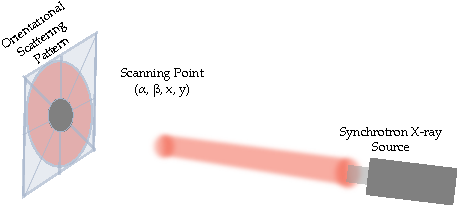
\includegraphics[width = 1\textwidth]{Figures/SAXSTT_annotated.pdf}
%     \caption{Experimental setup of a SAXS experiment. The beam canon represents the synchrotron beam. The cube represents a single row of voxels in the sample.
%         The scattering intensity from eight sectors of the diffractogram is collected for each scanning point $(\alpha, \beta,x,y)$.
%         Due to uniaxial symmetry, only one half of the diffractogram needs to be sampled. The half-circle is partitioned into 8 sector, meaning that the entire diffractogram is divided into 16 sectors of 22.5 degrees.}
%     \label{fig:experimental_setup}
% \end{figure}

%Figure of scanning orientations?


\section{Modelling of Anisotropic Scattering} \label{sec:modelling_scattering}
The coordinate systems used in this thesis follow the convention of the article "Small-angle X-ray scattering tensor tomography:
model of the three-dimensional reciprocal-space
map, reconstruction algorithm and angular
sampling requirements" \cite{liebi2018small}.
The reciprocal space map of a voxel is denoted $\vectorBU{\widehat{R}}(\vectorBU{r'}, \vectorBU{q'})$,
where $\vectorBU{r'}$ and $\vectorBU{q'}$ are the position and scattering vector in the object-coordinate system, respectively.
Transformation from the lab-coordinate system $\vectorBU{a}$ to the object-coordinate system $\vectorBU{a'}$ for a given property $\vectorBU{a}$
is given by the applying the rotation matrix $\vectorBU{R}_{n}^{exp}$ of the given projection $n$ with orientation $\left(\alpha,\beta\right)$.
Note that the properties often are higher order tensors, in which case the rotation matrix is applied so-called "page-wise",
meaning each matrix of the higher rank tensor is rotated separately.

% Fig to show alpha and beta. Thinking simple sphere with dots. 

One choice of representing the reciprocal space map is to model the form factor as a linear combination of spherical harmonics functions.
The reciprocal space map is then,
as given in Equation \eqref{eq:scattering_intensity_classical}:

\begin{equation}\label{eq:reciprocal_space_map}
    \vectorBU{\widehat{R}}(\vectorBU{r'}, \vectorBU{q'}) = \left\| \sum_{l, m=0} \vectorBU{a}_{l}^{0}(\vectorBU{r'}, q') \vectorBU{Y}_{l}^{0} \{ \Theta(\vectorBU{r'}, q'), \Phi(\vectorBU{r'}, q') \} \right\|^{2}.
\end{equation}

Equation \eqref{eq:reciprocal_space_map} only sums over the spherical harmonics functions $\vectorBU{Y}_{l}^{0}$ and coefficients $\vectorBU{a}_{l}^{0}(\vectorBU{r'}, q')$ with $m=0$,
since the nanostructures are assumed to have uniaxial symmetric reciprocal space maps.
As shown in Figure \ref{fig:spherical_harmonics}, the increasing even $l$-values of the spherical harmonics functions $\vectorBU{Y}_{l}^{0}$ correspond to highly oriented electron distributions.
The Figure also visualises the anisotropy using the unit sphere, and it is clear that only the pole of the sphere has significant scattering intensity for high even $l$-values.

\begin{figure}[h!]
    \centering
    \adjustbox{trim=0cm 0cm 0cm 0cm}{
        \includesvg[height=0.4\textwidth]{../XRD_CT/Plotting/plots/sph_harm_samples.svg}}
    \adjustbox{trim=0cm 1.5cm 0cm 1.5cm}{
        \includesvg[height = 0.4\textwidth]{../XRD_CT/Plotting/thesis_plots/sph_harm_spheres.svg}}
    \caption[Illustration of Spherical Harmonics]{Spherical harmonics functions $\vectorBU{Y}_{l}^{0}$ for some even $l$-values.
        They can be visualised as uniaxial structures or as an intensity distribution on the unit sphere.
        %RSD: Anything to say about the colours?
    }
    \label{fig:spherical_harmonics}
\end{figure}


Moreover, $q' = |\vectorBU{q'}|$ is the magnitude of the scattering vector $\vectorBU{q'}$, and $\Theta(\vectorBU{r'}, q')$ and $\Phi(\vectorBU{r'}, q')$ are the polar and azimuthal angles of the spherical harmonics function.
These angles may implicitly be defined by a series of coordinate transformations:

\begin{equation}\label{eq:coordinate_transformations}
    \begin{pmatrix}
        sin \Theta cos \Phi \\
        sin \Theta sin \Phi \\
        cos \Theta
    \end{pmatrix}
    = \vectorBU{R}^{str} \vectorBU{R}_{n}^{exp}
    \begin{pmatrix}
        sin \theta cos \phi \\
        sin \theta sin \phi \\
        cos \theta
    \end{pmatrix},
\end{equation}
\noindent
where $\vectorBU{R}^{str}$ is the rotation of the zenith of the spherical harmonics function in each voxel. The preferred orientation is parameterised by $(\theta_{op}, \varphi_{op})$.
The input is the spherical position coordinates in the lab-coordinate system $\vectorBU{r}$.
The rotation matrices in Equation \eqref{eq:coordinate_transformations} are defined as follows:
\begin{equation}
    \begin{split}
        \vectorBU{R}^{str}(\vectorBU{r'}) &=
        \begin{pmatrix}
            \costhetaop \cosphiop & \costhetaop \sinphiop & -\sinphiop  \\
            -\sinphiop            & \cosphiop             & 0           \\
            \sinthetaop \cosphiop & \sinthetaop \sinphiop & \costhetaop
        \end{pmatrix}\\
        \vectorBU{R}_{n}^{exp} &=
        \begin{pmatrix}
            \cos \beta & \sin \alpha \cos \beta & -\cos\alpha \sin\beta \\
            0          & \cos \alpha            & \sin \alpha           \\
            \sin\beta  & - \sin\alpha \cos\beta & \cos\alpha \cos\beta
        \end{pmatrix}
    \end{split}
\end{equation}

Alternatively, one could model the form factor using an exponential function where one parameter controls the amplitude, and the other controls the exponential decay,
which would account for the degree of anisotropy in this case. Uniaxial symmetry could be accounted for by a sinus squared term in the exponent.
Squaring the form factor function would give a reciprocal space map function on the form,
\begin{equation}\label{eq:exp_sin_squared}
    %\vectorBU{\widehat{R}}(\vectorBU{r'}, \vectorBU{q'}) = A^{2} \exp\{-B \sin^{2}\left( \Theta \right) \}, %RSD: What to do with parameters?
    %\vectorBU{\widehat{R}}(\vectorBU{r'}, \vectorBU{q'}) = \vectorBU{A}^{2}(\vectorBU{r'}, q') \exp\{-\vectorBU{B}(\vectorBU{r'}, q') \sin^{2}\left( \vectorgreek{\Theta}(\vectorBU{r'}, \vectorBU{q'}) \right) \},
    \vectorBU{\widehat{R}}(\vectorBU{r'}, \vectorBU{q'}) = \vectorBU{A}^{2} \exp\{-\vectorBU{B} \sin^{2}\left( \vectorgreek{\Theta} \right) \}, %RSD: Include r', q' as well?
\end{equation}
with resulting shape in threedimensional space as shown in Figure \ref{fig:exp_sin_squared}.

\begin{figure}
    \centering
    \adjustbox{trim=0cm 0cm 0cm 0cm}{
        \includesvg[height=0.4\textwidth]{../XRD_CT/Plotting/plots/exp_sin_samples.svg} }
    \adjustbox{trim=0cm 1.5cm 0cm 1.5cm}{
        \includesvg[height = 0.4\textwidth]{../XRD_CT/Plotting/thesis_plots/exp_sin_spheres.svg} }
    \caption[Illustration of Alternative Functional]{The function in Equation \eqref{eq:exp_sin_squared} for some sets of parameters (A,B).
        They can be visualised as uniaxial structures or as an intensity distribution on the unit sphere.}
    \label{fig:exp_sin_squared}
\end{figure}

There are a total of four parameters per voxel to optimise in Equation \eqref{eq:exp_sin_squared}: $A$, $B$, $\theta_{op}$, and $\varphi_{op}$.
In contrast, six parameters per voxel need to be optimised in Equation \eqref{eq:reciprocal_space_map},
$a_{0}$, $a_{2}$, $a_{4}$, $a_{6}$, $\theta_{op}$, and $\varphi_{op}$.
Moreover, the alternative representation provides the opportunity to model sharper directional scattering without the cost of additional optimisation parameters,
and the acuteness of the directional scattering can be adjusted in a continuous manner due to parameter $B$.
However, Equation \eqref{eq:reciprocal_space_map} is more general, and can be used to model a linear combination of isotropic and uniaxial intensities.


\section{Optimisation Algorithm}

SAXSTT is approximately a maximum likelihood estimation that can utilise gradient descent for optimisation, as mentioned in Chapter \ref{ch:optimisation}.
The forward pass of SAXSTT is to calculate the resulting SAXS patterns from the currently estimated model.
Then, the error between the calculated and measured SAXS patterns can be calculated.
In terms of cost function expressions, there exist many options, and the expression used by Liebi \cite{liebi2018small} is:
\begin{equation}\label{eq:cost_function_SAXSTT}
    \epsilon_{q} = 2 \sum_{n, x, y, \phi} \omega_{n}(x,y,q,\phi) \left\{ \left( \widehat{I}_{n}(x,y,q,\phi) \right)^{\frac{1}{2}}  -  \left( \frac{ I_{n}(x,y,q,\phi) }{T_{n}(x,y)} \right)^{\frac{1}{2}} \right\}^{2},
\end{equation}
\noindent
where the respective parts of the expression are a binary mask $\omega$, the calculated projection intensity $\widehat{I}_{n}$, the measured projection intensity $I_{n}$, and the transmission intensity $T_{n}$.
The latter accounts for absorption, which was another phenomenon, in addition to scattering, occurring when X-rays interact with matter,
as seen in Equation \eqref{eq:qm_interaction_Hamiltonian} in Chapter \ref{ch:scattering}. When using high energy X-rays, the absorption is negligible.

The calculated projection intensity $\widehat{I}_{n}$ can be estimated in a number of ways.
However, it is generally an interpolation from the estimated reciprocal space map $\vectorBU{\widehat{R}}$ to a set of projections.
Each SAXS projection $n$ can thus be expressed as a sum along the X-ray beam,
\begin{equation}\label{eq:SAXS_intensity}
    \widehat{I}_{n}(x,y,q,\phi) = \sum_{z} \reciprocalspacemap.
\end{equation}

Additional effort is recommended to ensure that the maximum likelihood estimation is converging towards the correct solution.
A separation of the optimisation into four steps was performed by Liebi \cite{liebi2018small} to ensure that the model was near convergence when optimising all parameters at once.
Therefore, the isotropic component $a_{0}$ is optimised first, followed by the preferred orientation $(\theta_{op}, \varphi_{op})$. In the second step, a guess of the uniaxial compontents has to be made.
Following this, the uniaxial components $a_{l}$ are optimised.
This allows the final optimisation to converge to a lower error value than if only one full optimisation were to be performed.


\section{Degree of Anisotropy} %RSD: Or Anisotropy?

A common measure for the degree of anisotropy is needed to quantify the results of SAXSTT.
The Hermans order parameter is common for describing the degree of anisotropy \cite{yoshiharu1997cellulose}.
The order parameter $S$ is defined as,
\begin{equation}\label{eq:hermans_order_parameter}
    S = \frac{1}{2} \left( 3 \langle\cos^{2} \Theta\rangle - 1 \right),
\end{equation}
where the average value of cosine squared is calculated by evaluating the integrals,
\begin{equation}
    \langle\cos^{2} \Theta\rangle = \frac{ \int_{0}^{\pi} f (\Theta) \cos^{2} \Theta \sin \Theta  \mathrm{d}\Theta  }
    {\int_{0}^{\pi} f (\Theta) \sin \Theta  \mathrm{d}\Theta },
\end{equation}
\noindent
where $f(\Theta)$ is the function, in which the average cosine squared value is to be calculated.
When referring to anisotropy for the remainder of this thesis, the Hermans order parameter will be used as the quantitative measure,
and uniaxial symmetry is implicitly assumed. %RSD?
% The degree of uniaxiality will be referred to as degree of anisotropy in the remainder of this thesis, for simplicity.

%RSD: Drop equatorial scattering?
\clearpage
\section{Scattering Models}

From the Hermans order parameter \eqref{eq:hermans_order_parameter}, it is clear that the possible interval of $S$ is $[-0.5, 1]$.
In the case of negative values, equatorial scattering is dominant, meaning that the resulting scattering is perpendicular to real-space orientation of the sample.
For positive values, the scattering is parallel to the real-space orientation of the sample, called meridional scattering.
To understand these phenomena, it is important to remember the properties of the Fourier transform.
Short length scales in real space correspond to high frequencies in reciprocal space, and vice versa.
When doing SAXSTT, only a limited \emph{q-range}, meaning a given frequency interval, is analysed.
The goal is to include either the meridional or equatorial scattering from the anisotropic sample.
If the characteristic length of the nanostructure is so that the corresponding scattering is found within the \emph{q-range},
but the same does not apply for the scattering from the width of the nanostructure, then only meridional scattering will be sampled.
Similarly can the opposite be true, where only equatorial scattering is sampled because the characteristic length of the nanostructure is too large.
Figure \ref{fig:scattering_models} shows the distinction between equatorial and meridional scattering.

\begin{figure}

    \centering
    \includegraphics[width=0.75\textwidth]{../XRD_CT/Figures/scattering_models.pdf}
    \caption[Meridional and Equatorial Scattering]{Meridional, or parallel, scattering is shown on the left, while equatorial, or perpendicular, scattering is shown on the right.
        The 3D figures in front represent objects in real space, while the respective sector diagrams directly behind the objects represent the corresponding scattering patterns for a certain \emph{q-range}.
        The characteristic length scales of the given \emph{q-ranges} are visualised by the dotted lines, respectively.
        For equatorial scattering, it is assumed that the length of the nanostructure corresponds to $q\sim0$.
        Therefore, only scattering from the width and the gap are sampled.
        Similarly, for meridional scattering, it is assumed that the width of the nanostructure causes wide-angle scattering, which is not sampled in the given \emph{q-range}.
    }
    \label{fig:scattering_models}
\end{figure}

Typically, equatorial scattering can occur when SAXS is performed on fibers \cite{li2013quantitative}, because X-rays scatter off the fiber-air interface.
This is also exemplified in Figure \ref{fig:scattering_models}.
Specifically, the mentioned interface has a characteristic length scale that is responsible for scattering intensity in the analysed \emph{q-range} of the SAXS data.
Moreover, scattering can also occur from the width of the fibers, given that the width and the gap are of similar size.
However, no meridional scattering is sampled, because the length of the fiber is too large to be sampled in the given \emph{q-range}.


